\documentclass[12pt,a4paper]{article}
\usepackage[UTF8]{ctex}
\usepackage{geometry}
\geometry{left=2.5cm,right=2.5cm,top=2.5cm,bottom=2.5cm}
\usepackage{graphicx}
\usepackage{amsmath}
\usepackage{amssymb}
\usepackage{booktabs}
\usepackage{array}
\usepackage{caption}
\usepackage{subcaption}
\usepackage{float}
\usepackage{siunitx}
\usepackage{listings}
\usepackage{xcolor}

\title{综合实验二：基于晶体管的温度传感器}
\author{严子竣，朱浩男，于耀博，郭健}
\date{\today}

\begin{document}

\maketitle

\section{引言}
本实验利用双极型晶体管基极-发射极电压差（$\Delta V_{\mathrm{BE}}$）与绝对温度成正比的物理特性（PTAT原理），构建一种高精度温度传感器。通过电流镜产生固定电流比，获取微弱的PTAT电压信号，再经差分放大和电平移位，将信号调理至适合ADC采集的0～5V范围，最终实现环境温度的数字显示。

\section{实验目的}
\begin{itemize}
    \item 建立传感器概念，培养综合应用电子电路的能力；
    \item 学习小型电子系统的设计、安装和调试方法；
    \item 培养工程实践中分析问题、解决问题的能力。
\end{itemize}

\section{电路设计}
整个系统分为两大部分：\textbf{测温前端}（PTAT电流镜）和\textbf{信号调理}（差分放大+电平移位）。如图1所示。

\begin{figure}[H]
    \centering
    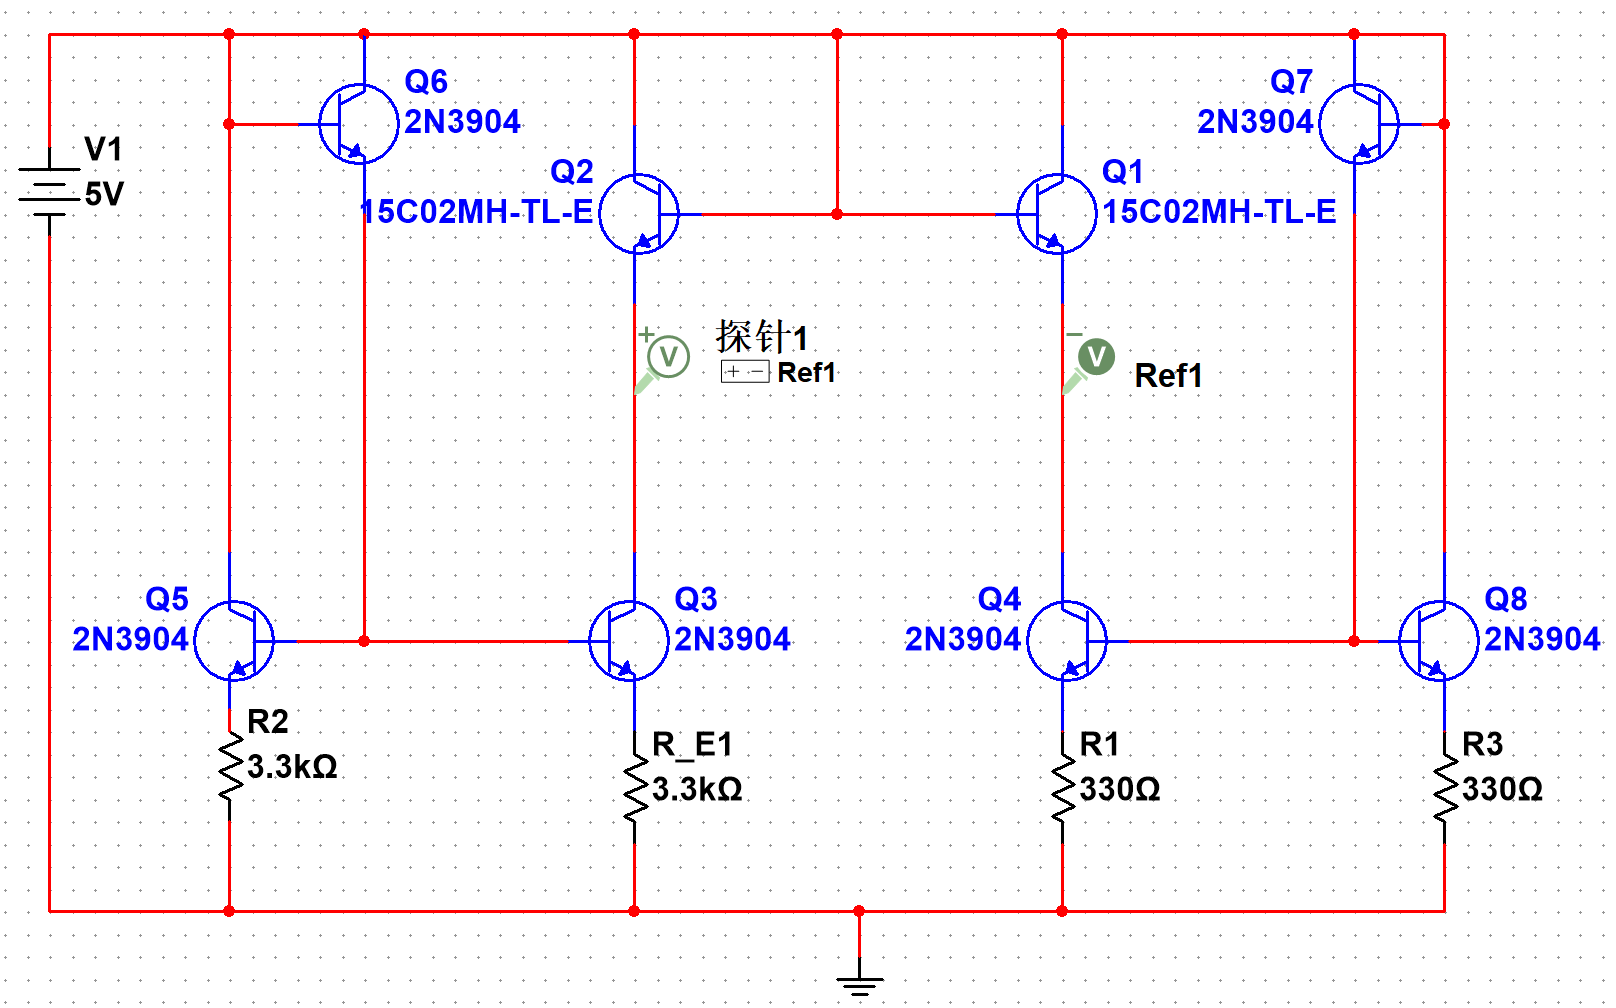
\includegraphics[width=0.45\textwidth]{temperature.png}
    \hfill
    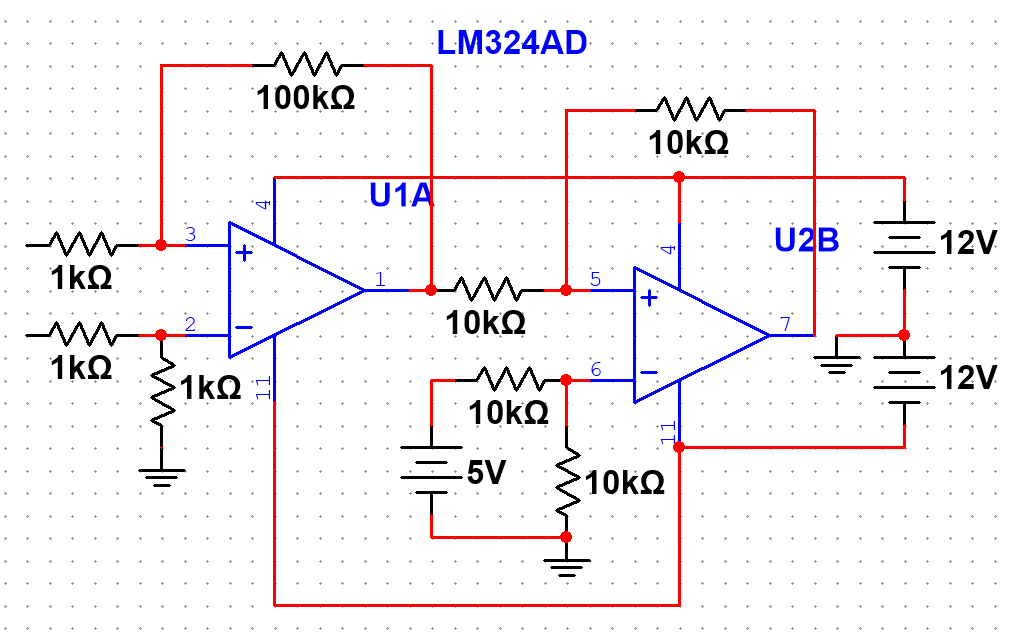
\includegraphics[width=0.45\textwidth]{amplification.png}
    \caption{左：带$\beta$-helper的电流镜（电流比约10:1）；右：LM324实现的差分放大与电平移位电路}
    \label{fig:circuits}
\end{figure}

左侧电路采用带$\beta$-helper的改进型电流镜，通过发射极电阻（$R_1=330\Omega$与$R_2=3.3\mathrm{k}\Omega$）设置两臂电流比约为10:1，从而在两只对管（Q1/Q2）的基-射极之间产生PTAT电压$V_{\mathrm{PTAT}}$。右侧电路第一级为差分放大器（增益约100倍），第二级为电平移位器，将输出的共模电平降低约5V，使其适配Arduino的0～5V ADC输入。

\section{理论计算}
\subsection{实测器件参数}
实际测得电流镜左右臂电阻上的电压分别为：
\begin{itemize}
    \item 右侧臂（$R=327.8\Omega$）：$V_R = 3.538\mathrm{V}$；
    \item 左侧臂（$R=3.271\mathrm{k}\Omega$）：$V_L = 3.660\mathrm{V}$。
\end{itemize}
由此计算两路集电极电流：
\begin{align}
    I_1 &= \frac{3.660}{3.271\times 10^3} = 1.119\times 10^{-3}\,\mathrm{A} \\
    I_2 &= \frac{3.538}{327.8} = 10.793\times 10^{-3}\,\mathrm{A}
\end{align}
电流比
\begin{equation}
    n = \frac{I_2}{I_1} = \frac{10.793}{1.119} \approx 9.646
\end{equation}
与设计值10吻合良好。

\subsection{PTAT电压温度系数}
根据半导体物理，PTAT电压满足
\begin{equation}
    V_{\mathrm{PTAT}} = \frac{kT}{q} \ln n
\end{equation}
其对温度求导得
\begin{equation}
    \frac{\mathrm{d}V_{\mathrm{PTAT}}}{\mathrm{d}T} = \frac{k}{q}\ln n
\end{equation}
其中 $\dfrac{k}{q} = 86.17\,\mu\mathrm{V/K}$。代入 $n=9.646$：
\begin{equation}
    \frac{\mathrm{d}V_{\mathrm{PTAT}}}{\mathrm{d}T} = 86.17\times 10^{-6} \times \ln(9.646) = 195.49\,\mu\mathrm{V/K}
\end{equation}
该值即为PTAT电压的理论温度灵敏度。

\subsection{放大后分辨率}
第一级差分放大增益实测 $A_v = 100.65$，则放大后的输出电压温度灵敏度为
\begin{equation}
    \frac{\mathrm{d}V_{\mathrm{out}}}{\mathrm{d}T} = A_v \cdot \frac{\mathrm{d}V_{\mathrm{PTAT}}}{\mathrm{d}T}
    = 100.65 \times 195.49\,\mu\mathrm{V/K} = 19.67\,\mathrm{mV/K}
\end{equation}
即每开尔文（摄氏度）温度变化对应19.67mV的输出电压变化，这是系统的理论分辨率。

\section{实际校准与测量范围}
使用商用数字温度传感器（DS18B20）作为参考，对设计系统进行两点校准。记录数据如下：
\begin{table}[H]
    \centering
    \begin{tabular}{c|c|c}
        \toprule
        温度（℃） & 输出模拟电压（V） & 备注 \\
        \midrule
        27.1 & 1.271 & 室温 \\
        110.0 & 2.928 & 热风枪加热 \\
        \bottomrule
    \end{tabular}
\end{table}

由两点计算实际灵敏度：
\begin{equation}
    \frac{\Delta V}{\Delta T} = \frac{2.928 - 1.271}{110.0 - 27.1} = \frac{1.657}{82.9} = 19.98\,\mathrm{mV/℃}
\end{equation}
该值与理论值19.67mV/K高度吻合，验证了设计的正确性。

根据校准直线（$V = 19.98\times 10^{-3} T + b$），由$T=27.1$时$V=1.271$求得截距$b = 1.271 - 19.98\times10^{-3}\times27.1 = 0.730\mathrm{V}$，即
\begin{equation}
    V = 0.01998\,T + 0.730
\end{equation}
反解温度：
\begin{equation}
    T = \frac{V - 0.730}{0.01998}
\end{equation}

Arduino ADC输入范围为0～5V，故可测量的温度范围为：
\begin{align}
    T_{\min} &= \frac{0 - 0.730}{0.01998} = -36.5\,℃ \\
    T_{\max} &= \frac{5 - 0.730}{0.01998} = 213.7\,℃
\end{align}
实际由于运放供电为$\pm12\mathrm{V}$，电平移位后最高输出可达5.5V，但受ADC量程限制，有效范围仍为0～5V，最终测量范围为 $-36.5℃ \sim 213.7℃$，可根据实际需求略微下调运放供电电压、增大差分放大倍数以进一步改进。

\section{电平移位的作用}
若不进行电平移位，差分放大器输出为双极性或共模电压较高，无法直接接入单极性ADC。通过第二级运放构建的电平移位电路：
\begin{itemize}
    \item 将输出电压整体下移约5V，使其落在0～5V区间；
    \item 充分利用ADC的满量程范围，避免因信号幅度过小导致量化误差占主导；
    \item 使得温度分辨率由简单的8位提升至接近10位（实际使用10位ADC），相比不移位方案分辨率提升约一倍。
\end{itemize}
本设计中，电平移位后的灵敏度约为20mV/℃，使得每℃对应约4个ADC码值（$5\mathrm{V}/1024 \approx 4.88\mathrm{mV}$），可分辨0.25℃的温度变化，满足精度要求。

\section{实验现象}

室温下测温电路与商用温度传感器相比，温度差距基本在$1^\circ$C以内；使用热风枪加热时，温度很快上升至$100^\circ$C以上，相比商用温度传感器温度上升较快，可能是由于商用温度传感器不考虑温度剧烈变化的情况，使用了较大的电容进行稳压。在热风枪下工作一段时间后，两温度计的温度都稳定在$106^\circ$C左右，且冷却后温度计仍与商用温度计相差$1^\circ$C以内，说明测温电路能够较为准确的测量温度。

\section{总结}
本文基于PTAT原理设计并实现了一款温度传感器，主要成果如下：
\begin{enumerate}
    \item 采用带$\beta$-helper的电流镜产生稳定的10:1电流比；
    \item 通过100.65倍差分放大和电平移位，将灵敏度提升至19.67mV/K，实际校准灵敏度为19.98mV/K，误差小于2\%；
    \item 理论有效测量范围覆盖$-36.5℃$至$213.7℃$，远超基本要求；
    \item 电平移位策略显著提高了ADC量程利用率，使得系统分辨率较简单放大方案提升一倍。
\end{enumerate}
实验表明，该方案具有成本低、线性度好、易于与数字系统接口等优点，具有较高的工程实用价值。

% ===== 在文档末尾（\end{document} 前）插入以下附录内容 =====
% 需要在导言区添加：\usepackage{listings} 和 \usepackage{xcolor}（可选）

\appendix
\section{Arduino 数据采集与显示代码}

以下为 Arduino 端完整程序，实现模拟传感器（A0）与数字参考传感器（DS18B20）的双通道采集，并经线性校准后显示于 OLED 屏幕。

\begin{lstlisting}[language=C++, caption=Arduino 测温程序, label=code:arduino]
#include <U8g2lib.h>
#include <Wire.h>
#include <OneWire.h>
#include <DallasTemperature.h>

// OLED 初始化 (硬件 I2C)
U8G2_SSD1306_128X64_NONAME_1_HW_I2C u8g2(U8G2_R0, 
    /* reset=*/ U8X8_PIN_NONE);

// ----- DS18B20 配置 -----
#define ONE_WIRE_BUS 8          // DQ 接 Arduino D2
OneWire oneWire(ONE_WIRE_BUS);
DallasTemperature sensors(&oneWire);

// ----- 温度标定参数（根据实际电路调整） -----
const float V_LOW    = 1.271;   // 低温校准点电压
const float Temp_LOW = 27.1;    // 低温温度
const float V_HIGH   = 2.928;   // 高温校准点电压
const float Temp_HIGH= 110;     // 高温温度
// -------------------------------------------

void setup() {
  u8g2.begin();
  sensors.begin();              // 初始化 DS18B20
}

void loop() {
  // ---------- 读取 A0 模拟传感器（软件滤波）----------
  const int NUM_SAMPLES = 20;
  long sum = 0;
  for (int i = 0; i < NUM_SAMPLES; i++) {
    sum += analogRead(A0);
  }
  int raw = sum / NUM_SAMPLES;

  // 转换为电压 (假设 Arduino 工作电压 5V)
  float voltage = raw * (5.0 / 1023.0);

  // 线性插值计算 T1（模拟传感器温度）
  float SCALE = (V_HIGH - V_LOW) / (Temp_HIGH - Temp_LOW);
  float T1 = (voltage - V_LOW) / SCALE + Temp_LOW;
  // ------------------------------------------------

  // ---------- 读取 DS18B20 温度 (T2) ----------
  sensors.requestTemperatures();
  float T2 = sensors.getTempCByIndex(0);
  if (T2 == DEVICE_DISCONNECTED_C) {
    T2 = -999.0;   // 传感器未连接时的错误标记
  }
  // ------------------------------------------------

  // ---------- OLED 显示 ----------
  u8g2.firstPage();
  do {
    // 第一行：T1（大字体）
    u8g2.setFont(u8g2_font_ncenB14_tr);
    u8g2.setCursor(0, 25);
    u8g2.print("T1: ");
    u8g2.print(T1, 1);
    u8g2.print(" C");

    // 第二行：T2（小字体）
    u8g2.setFont(u8g2_font_6x10_tr);
    u8g2.setCursor(0, 45);
    u8g2.print("T2: ");
    if (T2 == -999.0) {
      u8g2.print("Error");
    } else {
      u8g2.print(T2, 1);
      u8g2.print(" C");
    }

    // 第三行：A0 电压（小字体）
    u8g2.setCursor(0, 58);
    u8g2.print("A0: ");
    u8g2.print(voltage, 3);
    u8g2.print(" V");

  } while (u8g2.nextPage());
  // ----------------------------------

  delay(1000);   // 1秒刷新一次
}
\end{lstlisting}

\noindent 代码要点说明：
\begin{itemize}
    \item 采用20次均值滤波抑制随机噪声；
    \item 基于两点标定参数进行线性插值，将采集电压转换为温度；
    \item 同时读取DS18B20作为参考，用于实时比对校准；
    \item OLED 分三行显示模拟温度、参考温度和原始电压，刷新间隔1秒。
\end{itemize}
% ===== 附录结束 =====

\end{document}